% CREATED BY DAVID FRISK, 2018
\chapter{Introducción}

En este capítulo se presenta tanto el contexto como la motivación principal que ha impulsado todo el desarrollo de este proyecto. Además se resumen los objetivos del sistema desarrollado seguido de un resumen de la estructura de este mismo documento.

\section{Robótica}
\label{sec:robotica}

La robótica es la disciplina que engloba tanto el diseño como la  construcción y programación de robots. Esta disciplina no es aislada, ya que con ella se combinan muchas otras como la mecánica, electrónica, informática, inteligencia artificial o ingeniería de control. Citando a \textit{Robot Institute of America}, se puede decir que: "\textit{un robot es un dispositivo multifuncional reprogramable diseñado para manipular y/o transportar material a través de movimientos programados para la realización de tareas variadas}."

En esencia, un robot se compone de tres ingredientes fundamentales: sensores, actuadores y uno o más computadores. Podemos considerar un robot a toda aquella máquina o sistema informático que disponga de sensores: encargados de obtener la información del entorno que les rodea; actuadores: encargados de interactuar con dicho entorno; y uno o más computadores: encargados de ejecutar el software que analiza la información capturada por los sensores y genera señales correspondientes en los actuadores. Un último ingrediente que no se ha citado es el software. A pesar de no ser un elemento hardware, es la parte más importante de un robot, ya que es el encargado de dotar de un determinado comportamiento al mismo a través del procesamiento de información procedente de los sensores y la comanda de órdenes a través de los actuadores, utilizando como soporte un computador.

El primer robot programable y dirigido de forma digital data del año 1961. Diseñado por \textit{Unimate}\footnote{\href{http://www.prsrobots.com/unimate.html}{\texttt{http://www.prsrobots.com/unimate.html}}} éste primer robot realizaba tareas potencialmente peligrosas para humanos como levantar piezas calientes de metal de una máquina de tinte y colocarlas después correctamente.

\begin{figure}[htbp!]
	\begin{center}
		\subfloat[]{\label{fig:unimate}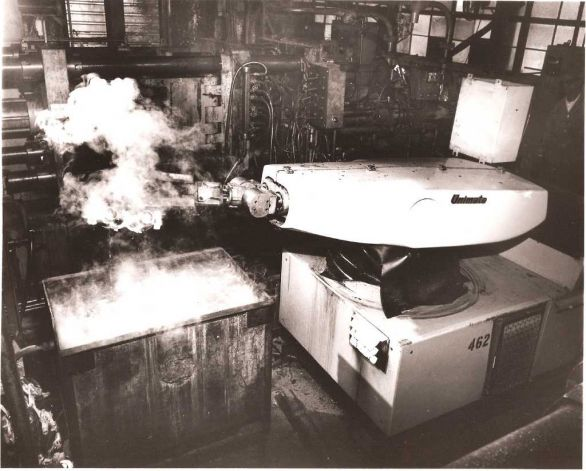
\includegraphics[width=.3\linewidth]{img/unimate}}
		\hspace{0.1cm}
		\subfloat[]{\label{fig:ancients}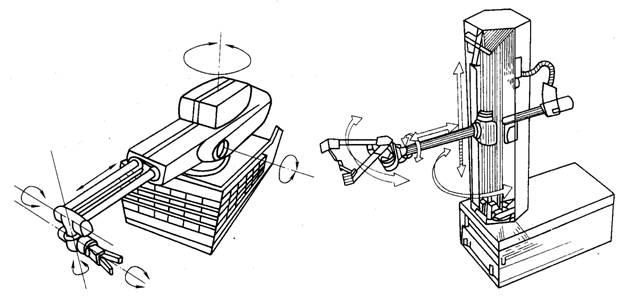
\includegraphics[width=.3\linewidth]{img/ancients_draw}}
		\hspace{0.1cm}
		\subfloat[]{\label{fig:versatran}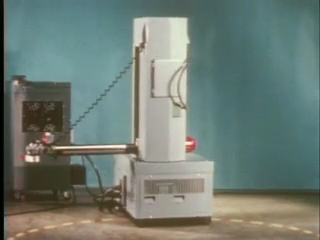
\includegraphics[width=.3\linewidth]{img/versatran}}
	\end{center}	
	\centering
	\captionsetup{justification=centering,margin=2.5cm}
	\caption{(a) Robot \textit{Unimate}, (b) esquemas del \textit{Versatran} y del \textit{Unimate} y (c) Robot \textit{Versatran}.}
	\label{fig:robots1}
\end{figure}

Esa fue la piedra angular que abrió el desarrollo masivo de diversos tipos de robot para todo tipo de usos. En los años siguientes, la robótica fue perfilándose hacia entornos más industrializados, debido a la creciente evolución del sector industrial. Es por ello que comenzaron a surgir robots orientados a la automatización de tareas repetetitivas, peligrosas para los humanos e incluso para tareas complejas que requieren de gran precisión. Algunos de los ejemplos más significativos de la época en cuanto a robots industriales puede ser el \textit{Versatran} (Figura \ref{fig:versatran}), el cual se desarrolló para el transporte de cargas, como su propio nombre indica \textit{Verstaile transfer} dentro de la fábrica de Ford en 1962.

Ya en 1969 se lanzan los primeros robots más característicos del mundo de la robótica: los robots soldadores. Estos robots surgen de la necesidad de precisión, y velocidad a la hora de realizar las soldaduras de los automóviles en las cadenas de producción de las fábricas. Además, cubrían aspectos tan importantes como la seguridad de los trabajadores, al considerarse el trabajo de soldadura como peligroso y dañino para las personas. Este tipo de robots aumentan en gran medida la productividad de las cadenas de producción debido a su alta precisión y velocidad. Un operario humano no podría desarrollar la misma tarea que desarrolla un robot soldador de forma tan fiable, tan rápida y tan segura.

Poco a poco los robots han ido evolucionando y a día de hoy tenemos robots con aptitudes muy diferentes y capaces de desarrollar tareas más complejas, no sólo en el campo de la investigación, sino en escenarios domésticos o industriales. Estos están muy presentes en tareas que resultan repetitivas, aburridas o peligrosas para los seres humanos. Buen ejemplo de ello son los robots que trabajan en la construcción de coches, pero también hay ejemplos en otros sectores como el de la bollería industrial con robots que se utilizan para embalar magdalenas (Figura \ref{fig:cupcake_robot}). Además, siguiendo la línea del entorno industrial, a parte de los ya mencionados robots han aparecido infinidad de robots para diferentes propósitos. Ya sea levantar cargas pesadas de forma autónoma, transporte de cargas y herramientas en un entorno controlado, o la simple tarea de embalar productos, como se acaba de mencionar. Uno de los ejemplos más claros a la hora de automatizar su funcionamiento es la empresa \textit{Amazon}, la cual cuenta con una flota de vehículos no tripulados encargados del transporte de mercancías dentro de sus naves industriales \footnote{\href{https://www.youtube.com/watch?v=tMpsMt7ETi8}{\texttt{http://www.youtube.com/watch?v=tMpsMt7ETi8}}}. Esta misma empresa está además contemplando la posibilidad de realizar entregas de paquetes en zonas de acceso complicado, como pequeños pueblos de montaña, mediante el uso de Drones, que se describen tres párrafos más abajo.

\begin{figure}
	\begin{center}
		\subfloat[]{\label{fig:beast}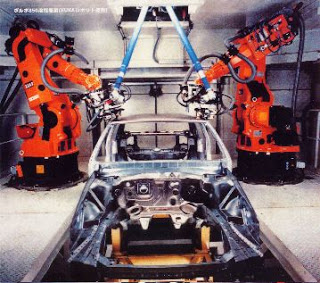
\includegraphics[width=.33\linewidth]{img/beast}}
		\hspace{0.1cm}
		\subfloat[]{\label{fig:stanford_cart}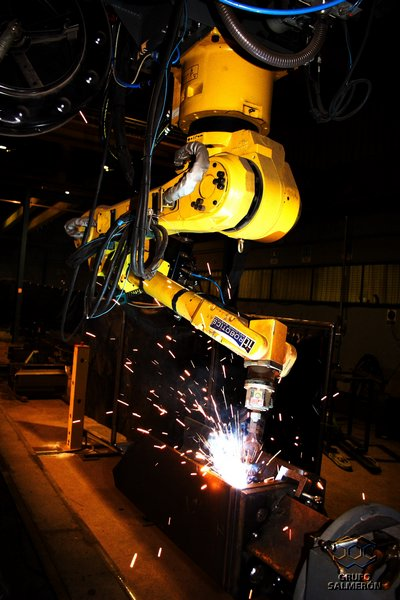
\includegraphics[width=.3\linewidth]{img/stanford_cart}}
	\end{center}	
	\centering
	\captionsetup{justification=centering,margin=0.1cm}
	\caption{(a) y (b) robots soldadores en plantas de producción industrial.}
	\label{fig:robots2}
\end{figure}

Actualmente, en el entorno doméstico, se comercializan robots muy útiles como el \textit{Roomba} de la empresa iRobot (Figura \ref{fig:roomba}). Este robot es un robot aspirador para las casas, pudiendo aspirar sobre cualquier superficie (suelo liso, azulejos, parqué, alfombras, etc.). Es un robot que posee diferentes sensores, de contacto e infrarrojos, y con un algoritmo de navegación se pasea por el suelo recogiendo el polvo, suciedad y residuos que encuentre a su paso.

El uso de \textit{UAVs} (\textit{Unmanned Aerial Vehicle} o vehículo aéreo no tripulado), o más comúnmente denominados \textit{drones} (Figura \ref{fig:drone}), cada vez está más extendido. En Alemania quieren usar este tipo de robots para defender los trenes de los grafiteros y el vandalismo, usándolos como medio de vigilancia en las cocheras. Con esta medida esperan ahorrar dinero, pues se estima en 10 millones de dólares anuales el gasto que supone limpiar los grafitis. Actualmente, en la Comunidad de Madrid se está estudiando el uso de robots de este estilo equipados con cámaras y sensores que detectan gases y agentes radiactivos para ayudar a los servicios de emergencia (bomberos, SAMUR y policía municipal) en labores de rescate, reduciendo no sólo costes sino también riesgos humanos. 

\begin{figure}
	\begin{center}
		\subfloat[]{\label{fig:cupcake_robot}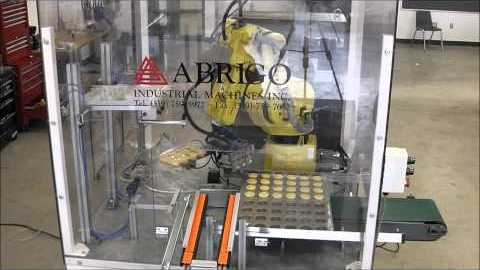
\includegraphics[width=.34\linewidth]{img/cupcake_robot}}
		\hspace{0.1cm}
		\subfloat[]{\label{fig:roomba}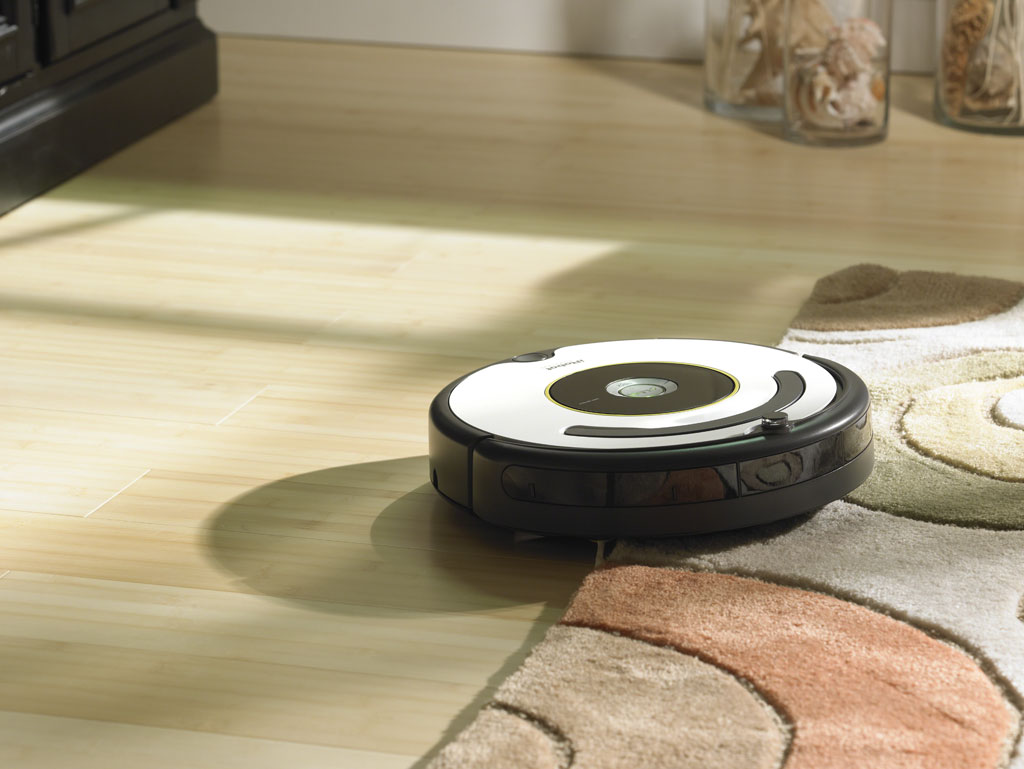
\includegraphics[width=.255\linewidth]{img/roomba}}
		\hspace{0.1cm}
		\subfloat[]{\label{fig:drone}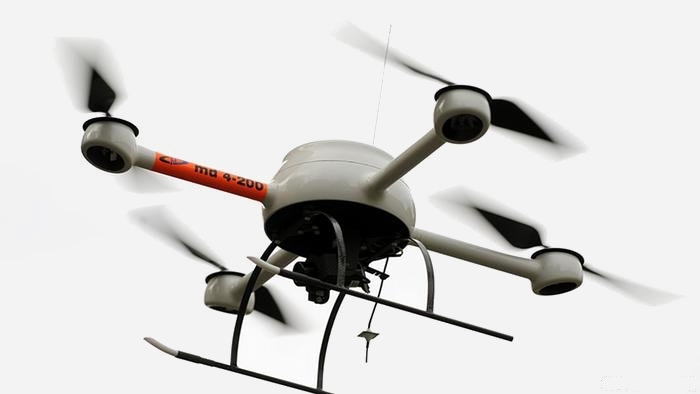
\includegraphics[width=.34\linewidth]{img/drone}}
	\end{center}
	\centering
	\captionsetup{justification=centering,margin=2cm}
	\caption{(a) Robot embalador de magdalenas, (b) \textit{Roomba} de iRobot y (c) robot aéreo no tripulado.}
	\label{fig:robots3}
\end{figure}

Por último, cabe mencionar que en la actualidad, la conducción autónoma se ha puesto a la cabeza de los problemas a investigar por parte de las empresas y de la comunidad científica. La conducción autónoma consiste en que un vehículo sea capaz de emular la capacidad de un humano de conducir tomando como información la proporcionada por diferentes sensores como cámaras de diversos tipos, láser tipo LIDAR, etc. El problema es complejo, ya que no sólo es necesario que el vehículo sea capaz de mantenerse dentro de la carretera, sino que además deberá cumplir con todas las normas de circulación pertinentes, al igual que debe hacer un humano. Es por esto que el problema aún no está resuelto, debido a su complejidad.

Existe un estándar realizado por la SAE (Sociedad de Ingenieros automotrices) que categoriza los niveles de conducción autónoma de un sistema en base a las capacidades del vehículo como se aprecia en la Figura \ref{fig:levelsdriving}:

\begin{enumerate}
    \item Nivel 0. No hay automatización; conduce un humano.
    \item Nivel 1. Asistencia al conductor. Algún sistema de apoyo como velocidad de crucero o autoaparcamiento. Sólo asiste al movimiento longitudinal o lateral.
    \item Nivel 2. Automatización parcial. El sistema puede tomar el control del vehículo en determinadas circunstancias controladas. No obstante el humano ha de supervisar en todo momento.
    \item Nivel 3. Automatización condicional. El sistema puede tomar decisiones en la conducción recibiendo información del entorno y calculando riesgos. El humano ha de intervenir cuando el sistema lo requiera.
    \item Nivel 4. Autonomía. El sistema tiene el control del vehículo; es capaz de detectar objetos y eventos y actuar ante ellos. 
    \item Nivel 5. Autonomía completa. No se requiere supervisión del humano; el sistema es capaz de realizar una conducción del vehículo en cualquier situación.
\end{enumerate}

\begin{figure}
  \centering
  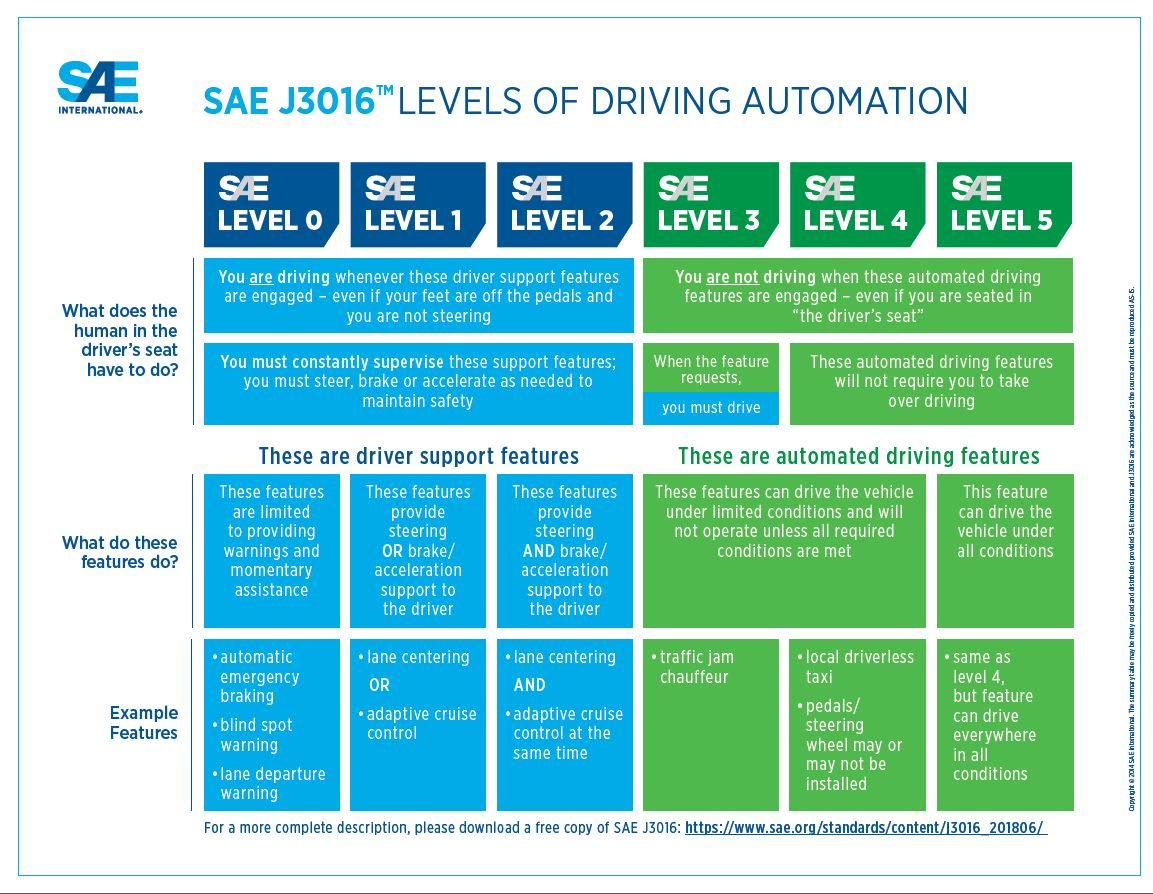
\includegraphics[width=.9\linewidth]{img/levels-of-driving}
  \caption{Niveles de conducción autónoma según el SAE}
  \label{fig:levelsdriving}
\end{figure}

Una de las empresas pionera en ofrecer soluciones a este problema de forma comercial es Tesla \footnote{\url{https://www.tesla.com}}, la cual desde hace ya algunos años comercializa vehículos con la tecnología necesaria para circular por una vía de forma autónoma, a la que han bautizado como \textit{AutoPilot}. No obstante, la empresa ofrece esta tecnología como un "asistente para la conducción" ya que, a pesar de que se ha demostrado que el coche es capaz de realizar la tarea, aún necesita la supervisión constante de un humano para evitar accidentes. Teniendo en cuenta la lista del SAE, se puede ver que la tecnología de Tesla está aún en el nivel 2, lo cual dista mucho aún de la conducción autónoma total.

El nivel más alto de esta lista lo tiene Google, con su proyecto Waymo. Teóricamente, Waymo está actualmente en el nivel 4 de la lista de SAE, aunque aún está en etapa de investigación. La tecnología de Waymo ha sido probada con éxito en diferentes entornos tanto de ciudad como de carretera de forma exitosa, no obstante, todas estas pruebas ha sido en entornos más o menos controlados.

En las siguientes secciones se explicará cómo conecta el problema de la conducción autónoma, la robótica, la visión artificial y el aprendizaje profundo, que son las tecnologías que enmarcan este proyecto.

\section{\textit{Deep Learning}}

El \textit{Deep Learning} o aprendizaje profundo es un campo dentro del aprendizaje automático (\textit{Machine Learning}), que utiliza estructuras de redes neuronales organizadas en capas para conseguir aprender representaciones de los datos más significativas conforme se avanza en las capas de la red. La palabra \textit{deep} hace referencia al número de capas que se utilizan en la red, por lo que se suele considerar que una red neuronal de más de 3 capas ya es una red neuronal profunda. Una red neuronal es un tipo de algoritmo que se caracteriza por emular el funcionamiento de un sistema nervioso humano, donde las diferentes neuronas conectadas entre sí trabajan juntas para solucionar un problema dentro de un dominio. La definición formal de una red neuronal es que es una función de aproximación de funciones universal, donde dada una entrada de datos que entra a un sistema se pueda obtener una determinada salida; por lo que una red neuronal no deja de ser una función.

En la Figura \ref{fig:simplenet} se ilustra una arquitectura de red neuronal básica. Esta red en particular consta de 3 capas: una capa de entrada, una capa oculta y una capa de salida. En la capa de entrada de datos representa los datos que ya han sido preparados para alimentar a la red en un formato determinado; la capa oculta se encarga principalmente de procesar la entrada de datos realizando los cálculos pertinentes para obtener una salida deseada actualizando los parámetros (pesos) de la misma; y la capa de salida que reciben los datos procesados por la red neuronal. Todas las neuronas en una capa están conectadas con alguna (o todas) neurona de la capa siguiente, y a cada neurona se le asigna un número llamado peso. El proceso de aprendizaje consiste principalmente en ajustar esos pesos para que dada una entrada de datos determinada, la red devuelva una salida esperada. Ese ajuste de pesos se realiza mediante ensayo-error de la siguiente manera: dada una entrada de datos, la red procesará dichos datos y generará una salida que será comparada con la salida ideal produciendo un error, ya que la salida de la red puede que no coincida exactamente con la salida esperada; el objetivo del aprendizaje de una red neuronal es que ese error se reduzca al máximo posible (idealmente el error será cero, ya que la salida de la red y la salida esperada serán la misma, por lo tanto la red no ha cometido errores), para ello cada vez que la red procesa una muestra de datos, ésta actualiza sus pesos mediante una técnica llamada \textit{back propagation}, que recibe su nombre por la forma en que propaga hacia atrás el error actualizando los pesos de la red mediante cálculos de derivadas sobre los mismos.


\begin{figure}
  \centering
  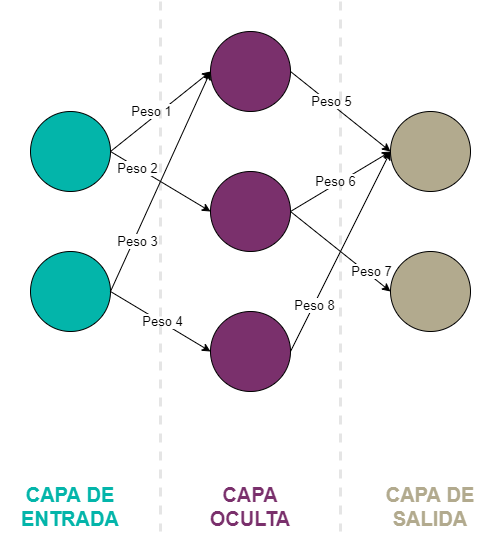
\includegraphics[width=.6\linewidth]{img/simplenet}
  \caption{Esquema de red neuronal sencilla}
  \label{fig:simplenet}
\end{figure}


Actualmente, los modelos más grandes tanto en tareas de visión artificial como de procesamiento de lenguaje natural (NLP) pueden tener cientos de capas.

En 2006 Geoffrey Hinton \cite{geoffreyhinton} propone un nuevo método de entrenamiento de las redes neuronales existentes hasta el momento, utilizando un entrenamiento por capas; de esta forma, cada capa de la red irá aprendiendo diferentes características de los datos de entrada empezando por las características más primitivas hasta las características más complejas extraídas de los datos según se avanza en las capas de la red. Este procedimiento se lleva a cabo hasta que se han entrenado todas las capas de la red. Este avance permitió el entrenamiento de redes mucho más profundas que las existentes en ese momento, popularizando el término \textit{deep learning} o aprendizaje profundo en castellano. Con el tiempo se ha demostrado que las redes neuronales más profundas otorgan resultados mucho mejores que otros modelos con menos capas o que las técnicas clásicas de \textit{machine learning}.

En la acutalidad la IA se encuentra en plena ebullición. Tanto es así que todas las empresas tecnológicas quieren implementar soluciones basadas en el \textit{deep learning} para sus productos y/o servicios. Así, las grandes empresas tecnológicas como Google, Amazon, Faceboo, Tesla, etc., ya ofrecen soluciones basadas en IA en diferentes campos como el NLP, la visión artificial o la robótica. Como ejemplos del último par de años tenemos el GPT-3 para generación automática de texto (OpenAI), Google Home y Amazon Echo Dot (Figura \ref{fig:homeecho}) con sus aistentes de voz inteligentes, Facebook utiliza el \textit{deep learning} para orientar sus anuncios e identificar objetos en las imágenes subidas por sus usuarios, Google con su buscador utiliza modelos de \textit{deep learning} con modelos basados en transformers para obtener mejores resultados en las búsquedas, incluso Amazon en sus almacenes con su flota de robots logísticos que utilizan \textit{deep learning} para moverse de forma eficiente por las naves o incluso Tesla y Google con sus proyectos de conducción autónoma basados en IA Autopilot\footnote{\url{https://www.tesla.com/autopilot}} y Waymo\footnote{\url{https://waymo.com}} respectivamente.

\begin{figure}
  \centering
  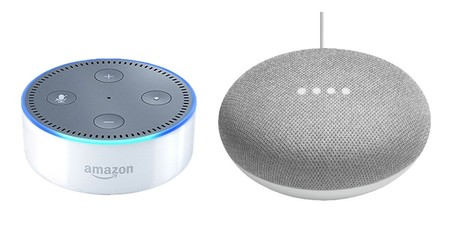
\includegraphics[width=.9\linewidth]{img/homeecho.jpg}
  \caption{Amazon Echo Dot y Google Home}
  \label{fig:homeecho}
\end{figure}


Una de las grandes compañías que han apostado por el \textit{deep learning} es Facebook. Con Yann LeCun a la cabeza en el laboratorio de IA de Facebook, se desarrolla DeepFace \cite{deepface} en 2014. DeepFace es un algoritmo basado en \textit{deep learning} que es capaz de reconocer rostros en imágenes digitales con la misma precisión que un humano.

Una empresa de nacimiento reciente es consecuencia de la explosión en la IA es OpenAI \footnote{\url{https://openai.com}}. Esta empresa fundada por el fundador de empresas como Tesla y SpaceX, Elon Musk, es una empresa de investigación de IA sin ánimo de lucro. Uno de sus mayores logros desde su fundación es la creación de sus modelos de generación de texto en lenguaje natural: GPT-2 y su actual versión GPT-3. Estos dos modelos utilizan arquitecturas Transformers (que provocaron la explosión del campo del procesamiento del lenguaje natural o NLP en 2018), que son modelos de redes neuronales mucho más potentes que las LSTM permitiendo obtener información contextual con mucho mayor alcance temporal. Los algoritmos GPT-2 y GPT-3 tienen como objetivo la generación de texto en lenguaje natural simulando a un humano. Es tal la potencia de dichos modelos, que a pesar de que OpenAI es una empresa de \textit{softwre libre}, no liberaron el modelo de GPT-2 por el peligro que suponía en la generación de noticias falsas o textos de odio de forma masiva. A día de hoy, y como ya sucedió en 2012 con el campo de la visión artificial, el campo del NLP ha explotado con la llegada de los Transformers y está en pleno auge; incluso Google implementa modelos basados en estas arquitecturas para su buscador en la actualidad.

\section{\textit{Deep Learning} aplicado a la robótica con visión}

\textcolor{red}{WIP}
Uno de los proyectos de visión aritificial más ambiciosos de la última década ha sido GoogleBrain, que surgió en 2012 de la mano de Jeff Dean y de Andrew Ng. Para este proyecto se desarrolló una red neuronal profunda que era capaz de detectar patrones en imágenes y vídeos de Youtube, llegando poco tiempo después a ser capaz de reconocer gatos en vídeos de Youtube analizando las imágenes de cada fotograma. Dos años más tarde, la empresa DeepMind es absorbida por Google. DeepMind es una empresa dedicada al mundo de los videojuegos utilizando técnicas de \textit{deep learning}. En 2016, DeepMind consiguió batir al mejor jugador del mundo en Go, Lee Sedol por 5 a 1, utilizando su algoritmo de \textit{deep learning} AlphaGo meidante jugadas "creativas" y "nunca vistas" según jugadores de Go profesionales. No obstante, un año después crearon AlphaGo Zero, que es igual de potente que el AlphaGo original, pero con la mejora de que es un sistema autodidacta, esto es, que ha aprendido por sí mismo a jugar al juego mediante aprendizaje por refuerzo jugando contra sí misma sin ningún tipo de información a priori. AlphaGo y AlphaGo Zero se basan en la visión para procesar las jugadas en cada turno, y tomar decisiones en función de la disposición de las fichas en el tablero.

* hablar de amazon warehouse

* hablar de aspiradores

* hablar de waymo
Uno de los proyectos más prometedores e interesantes para este trabajo es Waymo, de Google.




\section{Objetivos}

Una vez comprendido el contexto en el que se desarrolla este proyecto, a continuación se plantea y describe el problema abordado, así como la metodología aplicada al desarrollo \textit{software} de las soluciones propuestas.

El objetivo principal de este proyecto es conseguir un algoritmo de control visual para conducción autónoma basado en \textit{deep learning}, para posteriormente aplicar la solución a un robot pequeño en un entorno real. Además se propone el desarrollo de una plataforma para la ejecución de comportamientos neuronales orientado a la conducción autónoma bautizada como BehaviorStudio, que servirá como infraestructura para probar la solución aportada para el primer objetivo.

Para desarrollar este problema a priori complejo, se han dividido ambos objetivos en subobjetivos más abordables, para una mejor gestión del tiempo y una planificación más eficiente. Los puntos 3 y 4 están relacionados con el desarrollo de la plataforma BehaviorStudio, los puntos 5 y 6 con el desarrollo de la solución para la conducción autónoma, y los puntos 1, 2, 7 y 8 son comunes para ambos objetivos. Se detallan a continuación:

\begin{enumerate}
    \item Estudiar el estado del arte de redes neuronales, visión artificial y conducción autónoma para obtener una visión panorámica del problema a resolver y ayudar en la toma de decisiones para este proyecto.
    \item Estudiar el contexto previo a este proyecto mediante la lectura y la réplica del trabajo de fin de máster de Vanessa Fernández, proyecto en el que se basa este mismo, ampliando una de sus líneas futuras.
    \item Planificación y diseño de la plataforma BehaviorStudio, generando todos los diagramas y documentación pertinente para el desarrollo del \textit{software}. En esta etapa se generarán los diagramas UML del diseño, \textit{mockups} de la aplicación y los requisitos de la misma.
    \item Desarrollo de los diferentes componentes de la plataforma BehaviorStudio, generación de pruebas unitarias y confirmación del funcionamiento en entornos simulados.
    \item Adquisición y montaje del robot escogido como plataforma \textit{hardware} para la resolución del primer objetivo. Instalación de todas las herramientas necesarias para el desarrollo del proyecto.Pruebas de ensamblaje, teleoperación, conectividad y movilidad del robot. Probar que el montaje es correcto, que el módulo de comunicación Wi-Fi tiene conectividad adecuada, y que los motores del robot y las placas controladoras funcionan correctamente.
    \item Desarrollo del algoritmo de control visual basado en \textit{deep learning} centrado en el uso de redes neuronales convolucionales para el problema de regresión utilizando redes recurrentes y aplicarlo en el robot real.
    \item Integración de la solución para la conducción autónoma en la plataforma BehaviorStudio y pruebas para comprobar el correcto funcionamiento de todas las partes en un entorno real.
    \item Experimentación y evaluación de la solución conseguida sobre diferentes circuitos.
    
\end{enumerate}

\noindent Además de los objetivos arriba listados, se querrá satisfacer una serie de requisitos para considerar válido el desarrollo del proyecto. Estos requisitos son:

\begin{itemize}
    \item La plataforma BehaviorStudio deberá ofrecer un interfaz de usuario sencillo, intuitivo y usable. Además deberá ofrecer la posibilidad de mostrar la información sensorial en tiempo real.
    \item El robot deberá ser capaz de completar al menos una vuelta en cada circuito propuesto.
    \item La plataforma BehaviorStudio deberá funcionar indistintamente en entornos tanto simulados como reales.
    \item El proyecto al completo se desarrollará en Python utilizando las librerías de programación más novedosas como PyTorch y PyQt.
    \item Los algoritmos propuestos han de ser ágiles no tardando demasiado tiempo entre iteraciones para que el comportamiento de los robots sea reactivo y los movimientos más fluidos.
    \item Se utilizará el \textit{middleware} robótico ROS por la compatibilidad entre entornos reales y simulados y porque facilita las comunicaciones entre los diferentes componentes de la aplicación.
\end{itemize}

\section{Metodología}

Para la realización de este proyecto se ha optado por seguir un modelo de desarrollo en espiral basado en prototipos, ya que ambos objetivos de este proyecto se ajustan más a este tipo de metodología. El modelo en espiral se basa en la idea fundamental de repetir las mismas tareas iterativamente de forma que en cada iteración se aumenta la complejidad del proyecto, permitiendo la generación de prototipos funcionales al final de cada uno. Debido a que se esperaban cambios en los requisitos constantemente típicos en proyectos de investigación, se ha optado por este modelo que permite libertad a la hora de reajustar funcionalidades específicas en cada ciclo, además de hacer el proyecto escalable tanto en funcionalidad como en complejidad sin afectar al tiempo de desarrollo.

Todo esto sumando a la posibilidad de llevar un control por hitos al final de cada iteración además de las reuniones semanales realizadas durante todo el proceso de desarrollo, hacen de este modelo el ideal en nuestro proyecto, dado que cada reunión ofrece realimentación para lo hecho teniendo así en todo momento el proyecto bajo control.

Como herramienta asociada al proyecto, se ha dispuesto de un blog en la página de Github de Jderobot que sirve como cuaderno de bitácora donde plasmar todo lo hecho durante el proceso de desarrollo. Dicho blog se puede encontrar en \textcolor{red}{enlace al blog}.

El modelo en espiral se realiza por ciclos o iteraciones que corresponden a las diferentes fases del proyecto software. Cada ciclo se compone de cuatro fases principales, en las que se realizan diferentes tareas:

\begin{itemize}
    \item \textbf{Determinar los objetivos}. Se definen las necesidades que debe cumplir el \textit{software} a desarrollar en cada iteración, contemplando los objetivos finales. Esto hace que la complejidad del proytecto y el coste del ciclo avancen en función del tiempo.
    \item \textbf{Evaluar alternativas}. Se deben tener en cuenta las diferentes formas de llegar al objetivo proponiendo alternativas a los distintos elementos del proyecto. Además se deben considerar los riesgos que puedan existir e intentar reducirlos al máximo.
    \item \textbf{Desarrollar y verificar}. Teniendo en cuenta las alternativas propuestas en la fase anterio, se debe elegir la mejor de ellas y desarrollarla para llegar a los objetivos propuestos, para que finalmente el proyecto de ese desarrollo sea verificado con las pruebas pertinentes.
    \item \textbf{Planificar}. Con los resultados de las pruebas realizadas en la fase anterior, se ha de planificar la siguiente iteración revisando los posibles errores cometidos durante el ciclo actual y se comienza con un nuevo ciclo.
\end{itemize}


%%%%%%%%%%%%%%%%%%%%%%%%%%%%%%%%%%%%%%%%%%%%%%%%%%%%%%%%%%%%%%%%%%%%%%%%
\begin{comment}

\section{Motivación}

En estos últimos años la inteligencia artificial o IA ha explotado exponencialmente tanto en investigación, como en desarrollo. \todo{Definición de IA extensa}

Han sido especialmente notorios dos campos dentro de la IA: la visión artificial con su explosión en 2012 gracias a AlexNet \cite{alexnet} y el procesamiento del lenguaje natural (NLP por sus siglas en inglés) con su auge en 2018 con la creación de BERT \cite{devlin2018bert}. Este proyecto se enmarca dentro del primer campo: la visión artificial.

\subsection{Visión artificial}

La IA comprende multitud de ramas diferentes que se centran en diferentes campos: Procesamiento del lenguaje natural, Ingeniería del conocimiento, Minería de datos, Aprendizaje automático, Aprendizaje profundo, Visión artificial, etc. 

Este proyecto se basa en visión artificial, que trata de obtener significado (información relevante) de las imágenes a través de un procesamiento determinado, de tal forma que las máquinas que integren algoritmos de visión artificial sean capaces de emular el sistema visual humano tomando decisiones en función de lo que "ve" en cada momento, y actuar acorde a esa información.

En 2012, se inicia una revolución en el campo de la visión artificial con la llegada de AlexNet \textcolor{red}{REF paper alexnet? o abajo}. Alex Krizhevsky batió todos los récords de precisión en el problema de clasificación de imágenes en el torneo anual de \textit{ImageNet} en 2012 al proponer un modelo basado en redes neuronales convolucionales. Después de competir en el \textit{ImageNet Large Scale Visual Recognition Challenge} \footnote{http://image-net.org/challenges/LSVRC/}, AlexNet saltó a la fama. Logró un error del 15,3\%. en la tarea de clasificación de imágenes, que fue un 10,8\% más bajo que el del segundo puesto. Este resultado fue gracias a la profundidad del modelo que era necesaria para su alto rendimiento y al uso de las redes neuronales convolucionales (CNN). En 2012 este tipo de procesamiento era muy caro desde el punto de vista computacional, pero se hizo factible gracias al uso de las GPU (\textit{Graphic Processing Unit} o Unidades de procesamiento gráfico) durante el entrenamiento.
Tras este hito, el campo de la visión artificial explotó y comenzaron a surgir multitud de modelos novedosos que expandieron los límites del aprendizaje profundo mejorando las técnicas de aprendizaje automático que existían hasta el momento. Esta revolución dio pie a la resolución de diferentes tipos de problemas usando la visión artificial en campos como la industria (p.e.: detección de imperfecciones en cadenas de montaje), la robótica (p.e.: navegación autónoma), la medicina (p.e.: detección de cáncer de mama), etc.

\subsubsection{Aplicaciones de la visión artificial}

Este proyecto se basa en la visión artificial aplicada al campo de la robótica, por lo que algunas de los problemas más interesantes que se están estudiando en estos momentos son los siguientes:

\textcolor{red}{Mencionar el problema a resolver, del trabajo de Vane en simulación al trabajo de Vane en real.}

\end{comment}


\begin{comment}
This chapter presents the section levels that can be used in the template. 

\section{Section levels}
The following table presents an overview of the section levels that are used in this document. The number of levels that are numbered and included in the table of contents is set in the settings file \texttt{Settings.tex}. The levels are shown in Section \ref{Section_ref}.

\begin{table}[H]
\centering
\begin{tabular}{ll} \hline\hline
Name & Command\\ \hline
Chapter & \textbackslash\texttt{chapter\{\emph{Chapter name}\}}\\
Section & \textbackslash\texttt{section\{\emph{Section name}\}}\\
Subsection & \textbackslash\texttt{subsection\{\emph{Subsection name}\}}\\
Subsubsection & \textbackslash\texttt{subsubsection\{\emph{Subsubsection name}\}}\\
Paragraph & \textbackslash\texttt{paragraph\{\emph{Paragraph name}\}}\\
Subparagraph & \textbackslash\texttt{paragraph\{\emph{Subparagraph name}\}}\\ \hline\hline
\end{tabular}
\end{table}

\section{Section} \label{Section_ref}
\subsection{Subsection}
\subsubsection{Subsubsection}
\paragraph{Paragraph}
\subparagraph{Subparagraph}

\end{comment}